\subsection{Analyse und Aufbereitung}
\label{sec:AnalyseAufbereitung}

Ziel dieses Abschnitts ist es, sich mit dem Datensatz vertraut zu machen und ihn aufzubereiten, sodass beispielsweise ungültige Einträge gelöscht werden.
Außerdem ist es sinnvoll, einige Analysen durchzuführen.
Dies führt zu einem besseren Verständnis des Datensatzes und legt etwaige Inkonsistenzen offen.

Der von der Eifrig Media GmbH bereitgestellte Datensatz liegt als sql-Datei vor.
Für die Weiterverarbeitung muss die Datei in eine MySQL oder MariaDB Datenbank eingelesen werden.
Die Datenbank kann komfortabel mit Docker erstellt werden.
Eine entsprechende Docker-Compose Datei mit einer MariaDB Instanz und weiteren Komponenten, die im Verlauf dieses Abschnitts benötigt werden, befindet sich in \appendixref{sec:AnhangDockerCompose}.
Als grafische Oberfläche für den Zugriff auf die Datenbank enthält die Docker-Compose Datei außerdem eine phpMyAdmin Instanz.

Der Datensatz beinhaltet 7.787.865 Meldungen und deckt den Zeitraum vom 22.05.2014 bis 25.10.2021 ab. Dies entspricht ca. 21.300 Meldungen pro Tag.
Bei Betrachtung des Datensatzes fällt zunächst auf, dass einige Meldungen Inkonsistenzen aufweisen:

\begin{itemize}
    \setlength\itemsep{-15pt}
    \item 1160 Meldungen haben als Aufbauzeitpunkt den ungültigen Wert "`0000-00-00 00:00:00"'.
    \item Bei 420 Meldungen liegt der Abbauzeitpunkt vor dem Aufbauzeitpunkt.
    \item Bei 9800 Meldungen beträgt die Standdauer 20 Minuten oder weniger.
    % Der angemerkte Punkt steht schon hier: ;)
    \item Bei 62.000 Meldungen beträgt die Standdauer mehr als 24 Stunden, bei 1960 mehr als ein Jahr.
\end{itemize}

Da der Anteil an Meldungen mit ungültigem Auf- oder Abbaudatum nur 0,02\,\% beträgt, bietet es sich an, diese Meldungen aus dem Datensatz zu entfernen.
Auch die Meldungen mit einer sehr geringen Standdauer von 20 Minuten oder weniger sollten entfernt werden, da es sich hierbei vermutlich um Fehlmeldungen handelt.
Nun stellt sich die Frage, wie mit Meldungen umgegangen werden soll, die eine sehr lange Standdauer aufweisen.
Da sich im Datensatz 1962 Meldungen befinden, deren Standdauer über ein Jahr beträgt, ist davon auszugehen, dass die Standdauer einiger Meldungen im Datensatz falsch ist.
Dieses Argument lässt sich bekräftigen, wenn \autoref{fig:StanddauerVerteilung} betrachtet wird.

\begin{figure}[h]
    \centering
    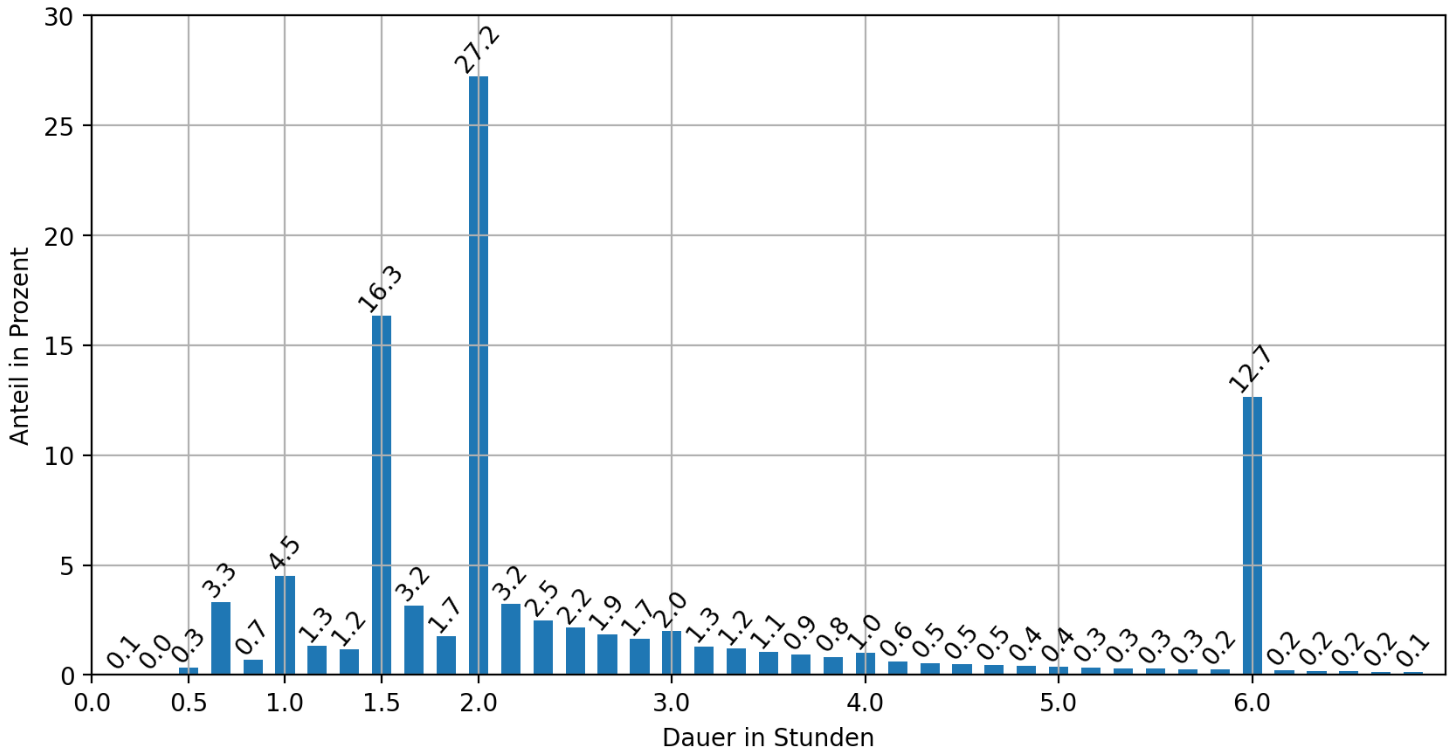
\includegraphics[width=1.0\textwidth,height=10cm,keepaspectratio=true]{content/images/Standdauer.png}
    \caption{Verteilung der Standdauer mobiler Radarkontrollen}
    \label{fig:StanddauerVerteilung}
\end{figure}

Es ist erkennbar, dass allein 56,1\,\% aller gemeldeten Radarkontrollen eine Standdauer von anderthalb, zwei oder sechs Stunden haben.
Insgesamt 97,45\,\% haben eine Standdauer von sieben Stunden oder weniger.
Damit liegt die Standdauer eines Großteils der Radarkontrollen bei wenigen Stunden.
Außerdem kann nicht belegt werden, dass schon eine Standdauer von mehr als 12 Stunden in der Realität auftritt.
Der Datensatz enthält jedoch ca. 91.000 Meldungen, auf die dieses Kriterium zutrifft.
Dies entspricht einem Anteil von 1,1 \,\%, was zu groß ist, um diese Meldungen komplett aus dem Datensatz zu entfernen.
Die bevorzugte Alternative besteht darin, den Abbauzeitpunkt aller dieser Meldungen auf 12 Stunden nach dem Aufbauzeitpunkt zu setzen.

Eine weitere Inkonsistenz des Datensatzes fällt auf, wenn die Anzahl der Meldungen pro Tag über den gesamten verfügbaren Zeitraum betrachtet werden.
Diese Metrik ist in \autoref{fig:AnzahlProTagAllData} dargestellt.

\begin{figure}[h]
    \centering
    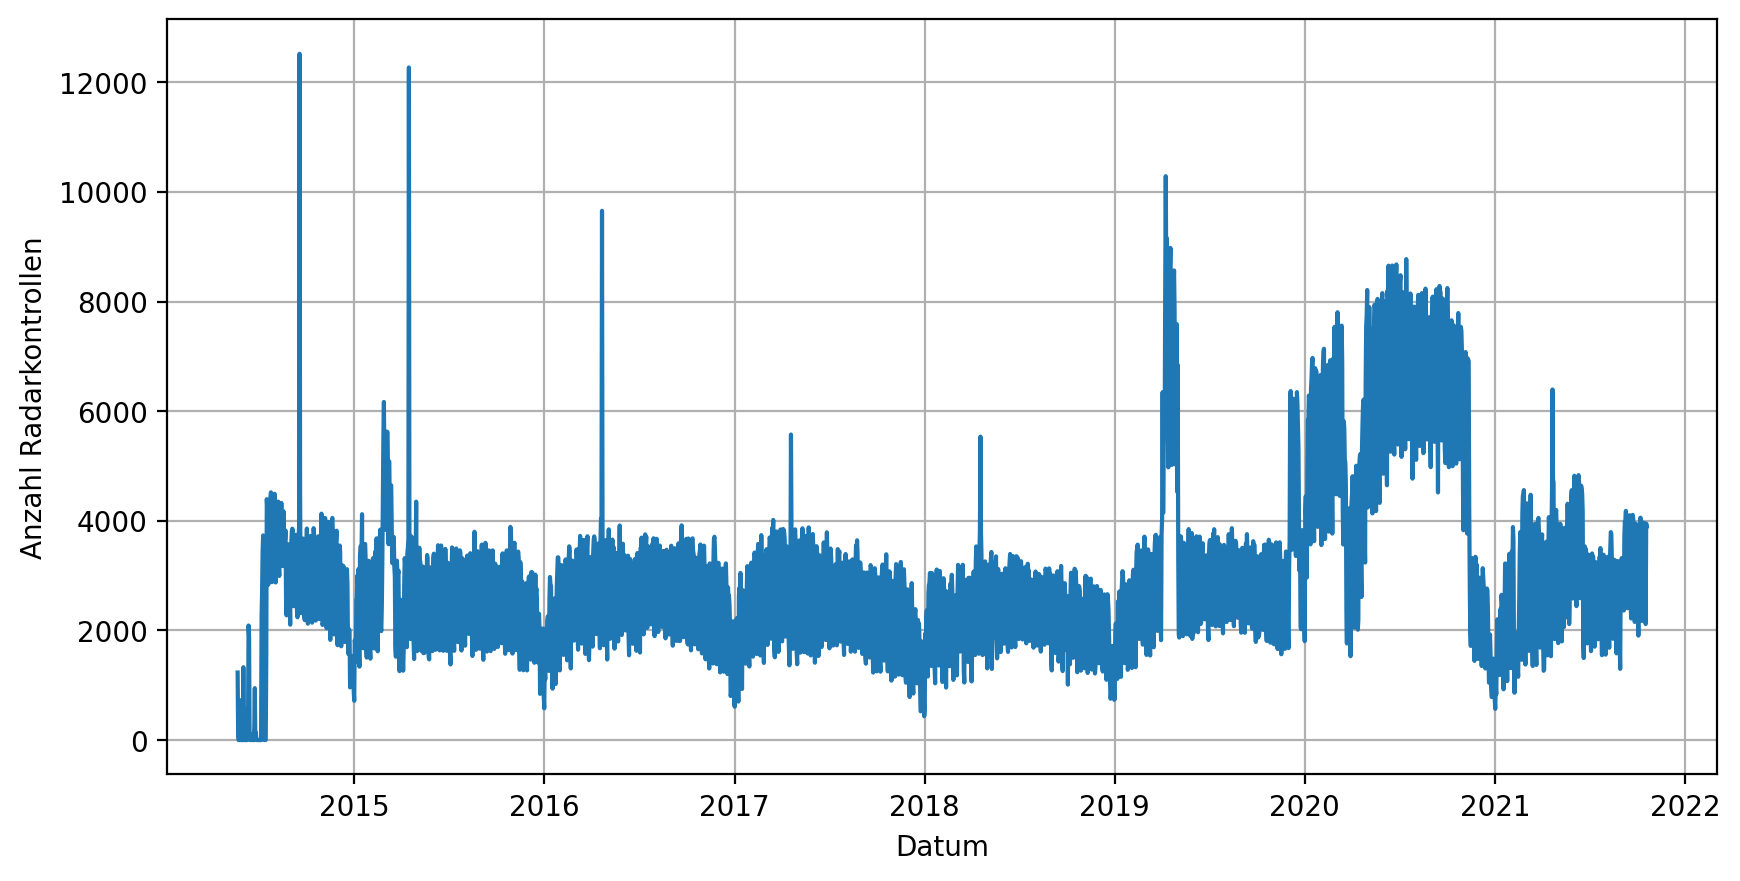
\includegraphics[width=1.0\textwidth,height=10cm,keepaspectratio=true]{content/images/AnzahlProTagAllData.png}
    \caption{Anzahl mobiler Radarkontrollen pro Tag vom 22.05.2014 bis 20.10.2021}
    \label{fig:AnzahlProTagAllData}
\end{figure}

Es fällt auf, dass deutlich weniger Meldungen im Zeitraum vom 22.05.2014 bis zum 16.07.2014 vorhanden sind als in den Jahren danach.
Das spricht dafür, dass der Datensatz in diesem Zeitraum unvollständig ist.
Da dies das Training des \acrshort{nn}s negativ beeinflussen würde, sollten alle Meldungen vor dem 17.07.2014 aus dem Datensatz entfernt werden.
In \autoref{fig:AnzahlProTagAllData} sind noch einige weitere interessante Muster zu erkennen.
Zunächst gibt es einige sehr schmale Ausschläge.
Beispielsweise waren am 17.09.2014 3800 mobile Radarkontrollen aufgestellt, am 18.09.2014 dann 12.400 und am 19.09.2014 wieder nur 4140.
Diese Ausschläge sind je auf einen sogenannten "`Blitzermarathon"' zurückzuführen, bei denen an einem bestimmten Tag besonders viele Radarkontrollen aufgestellt werden.
Ein Vergleich der Radarkontrollen auf einer Karte zwischen dem Blitzermarathon am 18.09.2014 und dem Vortag befindet sich in \appendixref{sec:AnhangDiagramme}, \autoref{fig:BlitzerMarathonSep2014Vgl}.

Als Nächstes ist an \autoref{fig:AnzahlProTagAllData} noch auffällig, dass es eine jährliche Periodizität gibt.
Außerdem bleibt die durchschnittliche Anzahl an Radarkontrollen pro Jahr annähernd konstant, wenn der Ausschlag im Jahr 2020 außer Acht gelassen wird.
Das spricht dafür, dass der Datensatz vermutlich nicht durch eine sich verändernde Nutzerzahl verzerrt ist.
Es ist auch erkennbar, dass es im Sommer mehr mobile Radarkontrollen gibt als im Winter.
Dies geht auch aus \autoref{fig:AnzahlNachMonat} hervor, in der die Anzahl mobiler Radarkontrollen pro Monat dargestellt ist.

\begin{figure}[h]
    \centering
    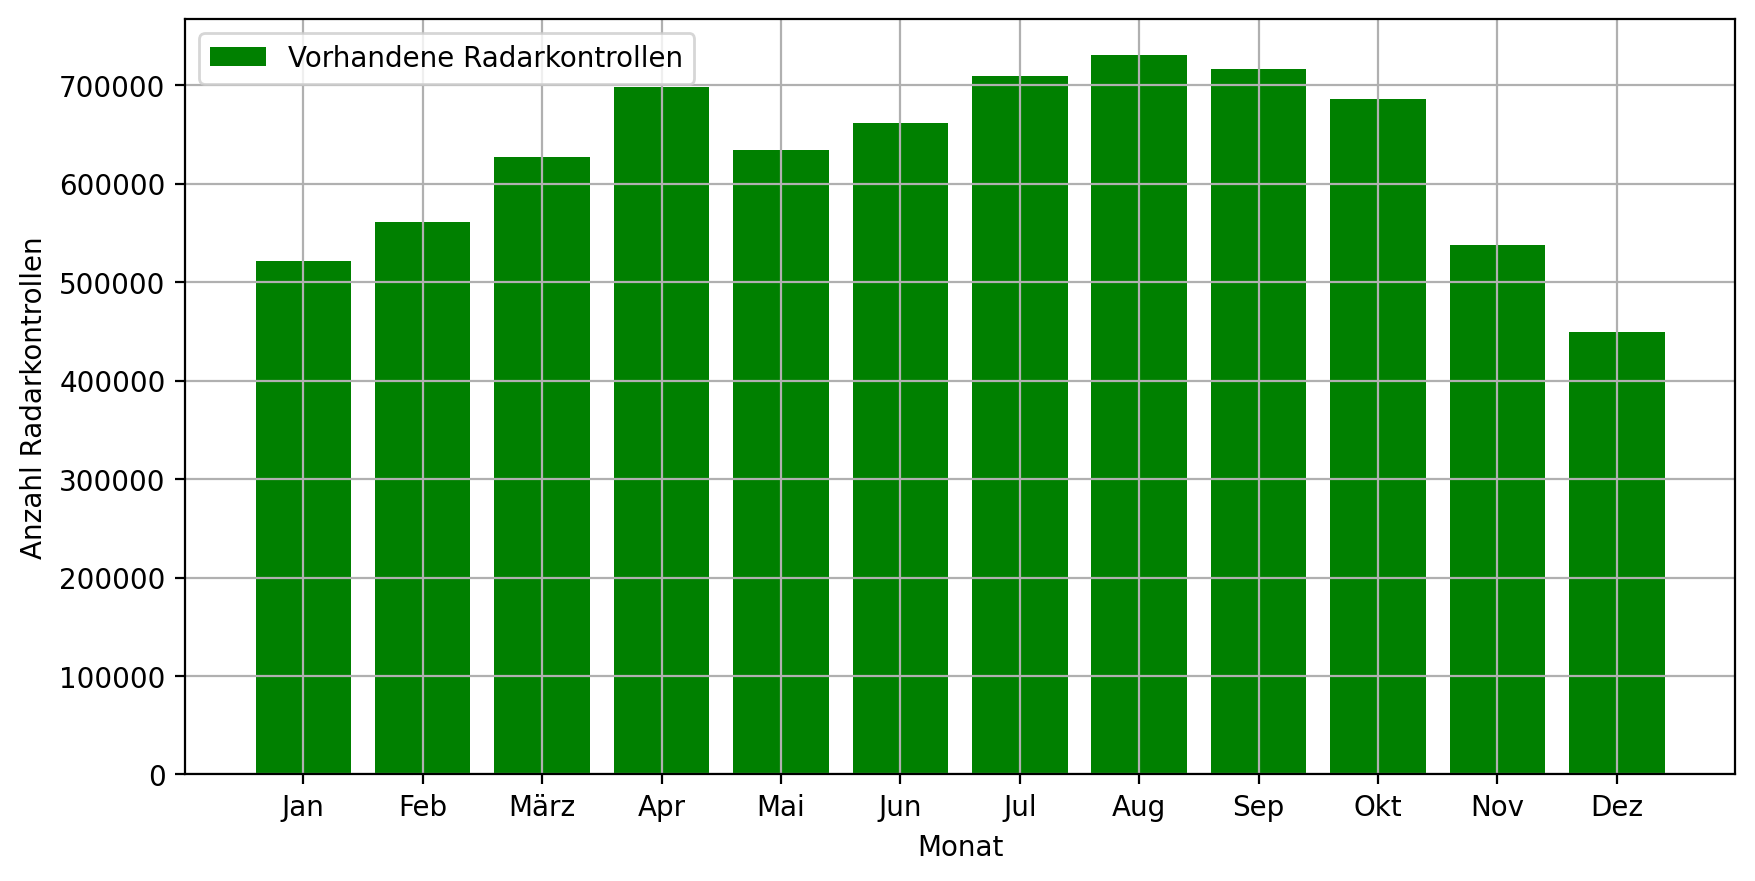
\includegraphics[width=1.0\textwidth,height=10cm,keepaspectratio=true]{content/images/AnzahlNachMonat.png}
    \caption{Anzahl mobiler Radarkontrollen nach Monat}
    \label{fig:AnzahlNachMonat}
\end{figure}

Außerdem besteht eine wöchentliche Periodizität, die in \autoref{fig:AnzahlProTagAllData} aufgrund der begrenzten Auflösung nicht erkennbar ist.
Daher ist in \autoref{fig:AnzahlNachWochentag} die Anzahl mobiler Radarkontrollen pro Wochentag in Rot dargestellt.

\begin{figure}[h]
    \centering
    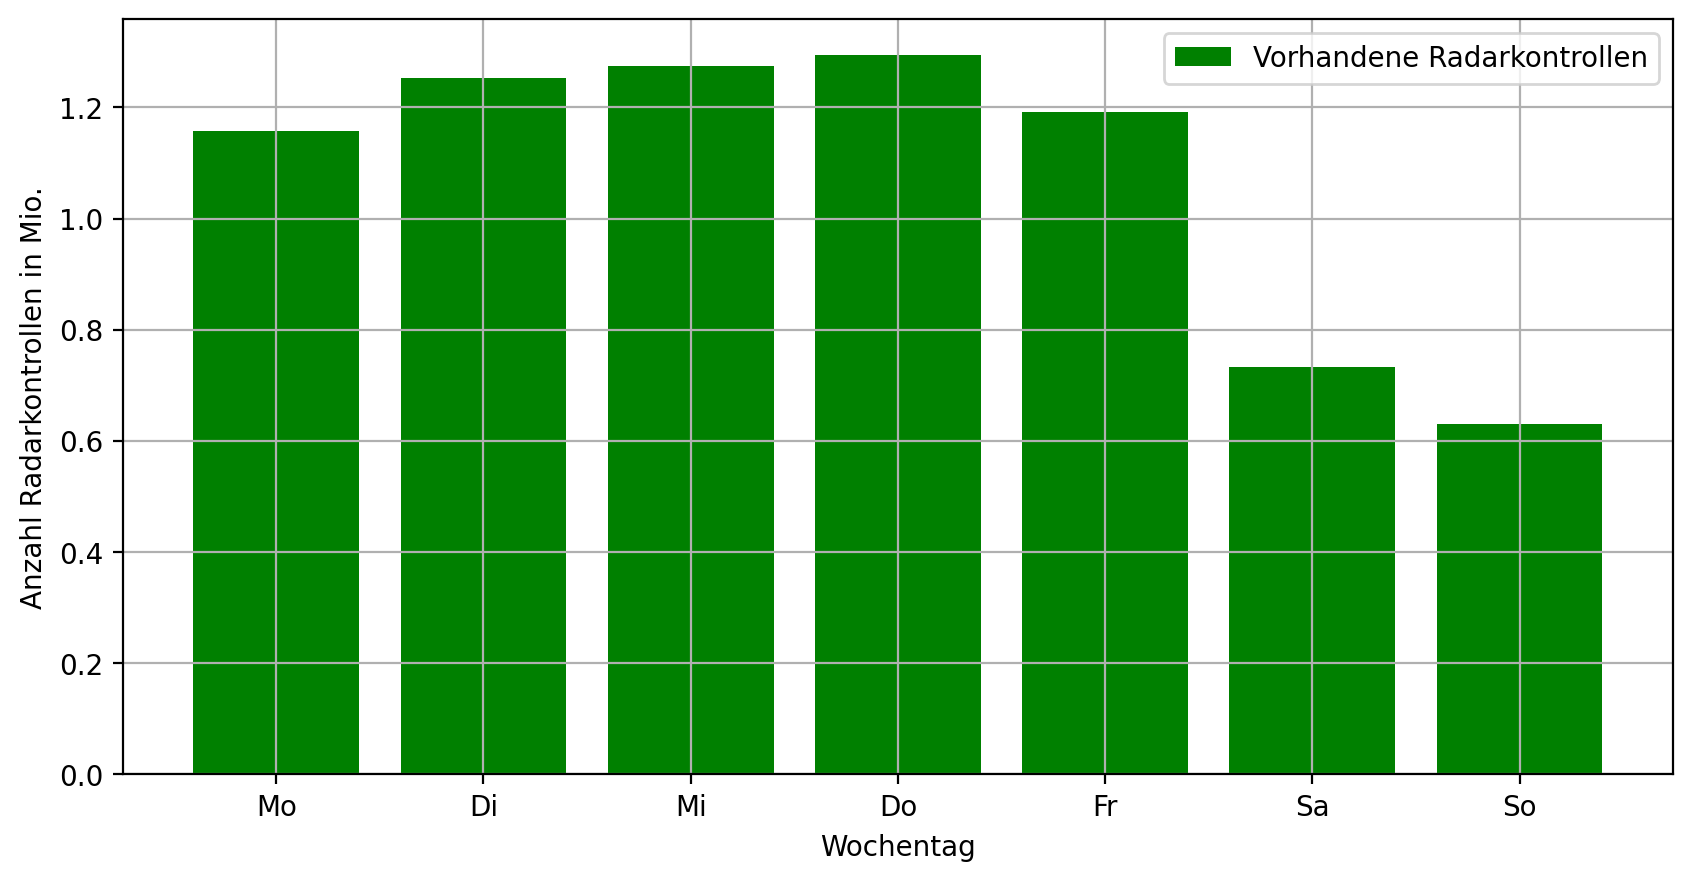
\includegraphics[width=0.8\textwidth,height=8cm,keepaspectratio=true]{content/images/AnzahlNachWochentag.png}
    \caption{Anzahl mobiler Radarkontrollen nach Wochentag im Vergleich zur durchschnittlich gefahrenen Tagesstrecke pro mobiler Person. Die Tagesstrecke stammt aus \cite[Tabelle 3]{MiD}.}
    \label{fig:AnzahlNachWochentag}
\end{figure}

Es fällt auf, dass am Wochenende pro Tag nur ca. halb so viele Meldungen vorhanden sind wie unter der Woche, während die gefahrene Tagesstrecke \cite[Tabelle 3]{MiD} (in Grün dargestellt) ähnlich groß ist.
Dadurch lässt sich das Argument bekräftigen, dass die Anzahl an Meldungen nicht signifikant vom Verkehrsaufkommen und damit der Anzahl an Appbenutzern abhängig ist.

Bisher wurde der Datensatz hauptsächlich über zeitliche Auflösungen von über einem Tag analysiert.
Jedoch sind auch Statistiken interessant, die sich auf die Tageszeit beziehen.
So ist in \autoref{fig:AnzahlNachTageszeit} beispielsweise dargestellt, wie viele Radarkontrollen es je nach Tageszeit gibt.

\begin{figure}[h]
    \centering
    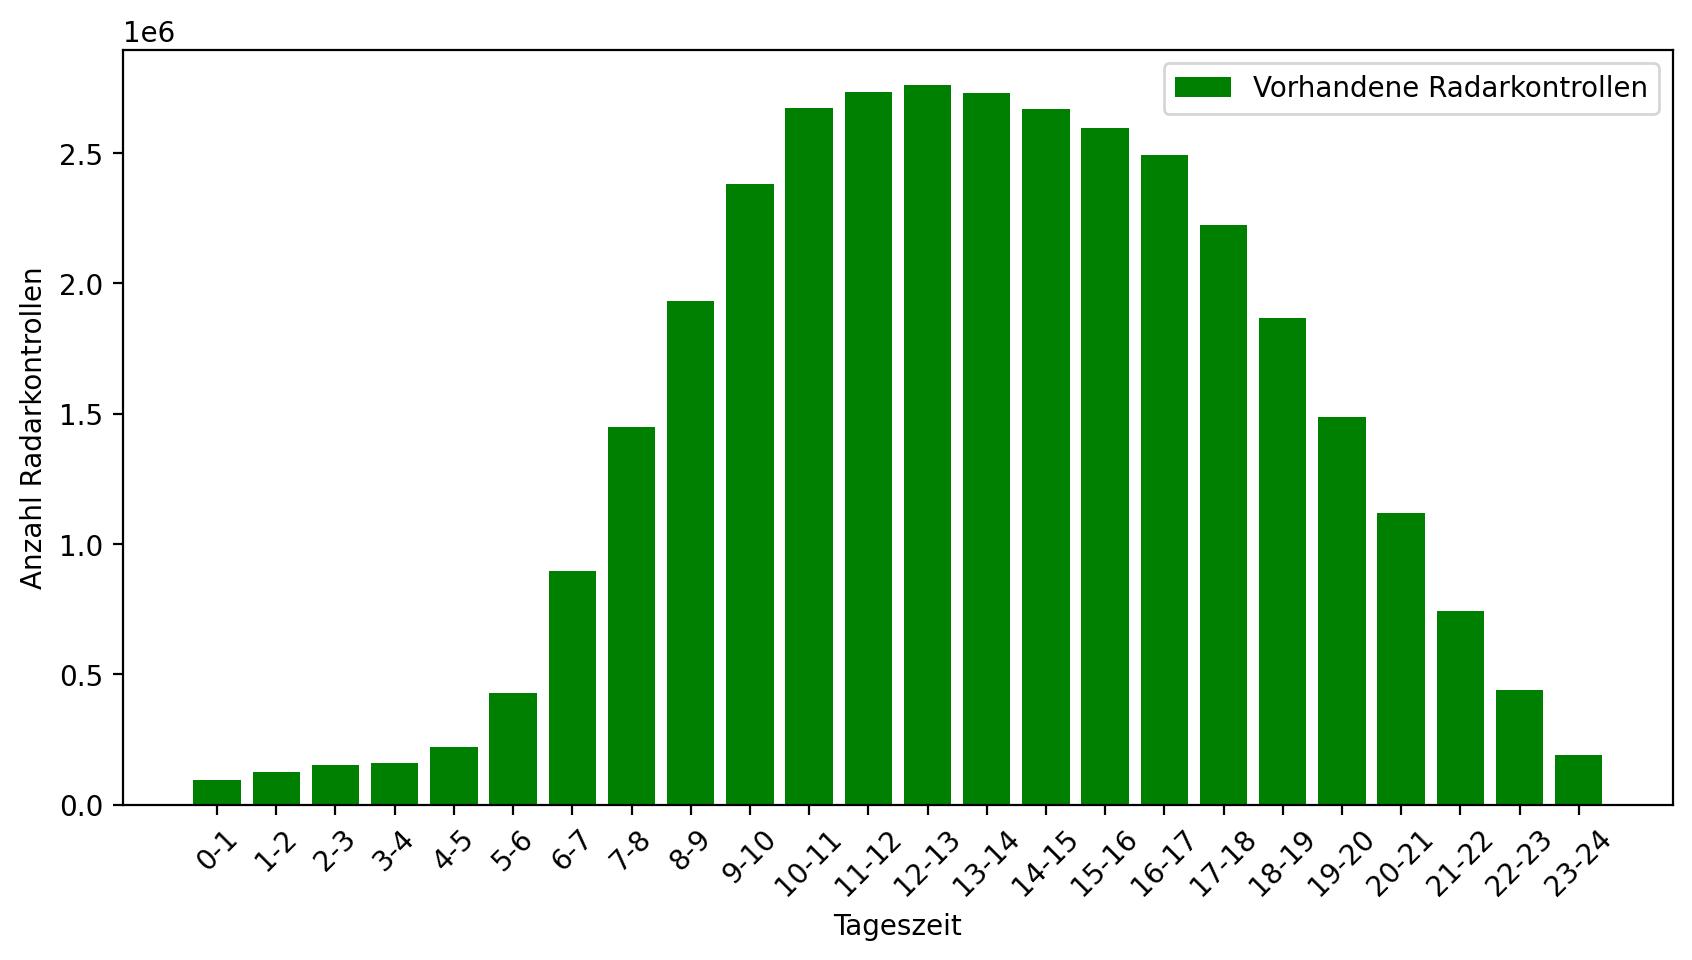
\includegraphics[width=1.0\textwidth,height=10cm,keepaspectratio=true]{content/images/AnzahlNachTageszeit.png}
    \caption{Anzahl mobiler Radarkontrollen nach Tageszeit}
    \label{fig:AnzahlNachTageszeit}
\end{figure}

Es fällt zunächst auf, dass es sich nicht um eine Gleichverteilung handelt.
Nachts (von 21 bis 6 Uhr) sind deutlich weniger Radarkontrollen vorhanden als tagsüber.
Um die Mittagszeit erreicht die Anzahl der Radarkontrollen ihren Höhepunkt, um Mitternacht ihren Tiefpunkt.
Der starke Anstieg zwischen 6 und 10 Uhr unterstreicht nochmals die Motivation dieser Arbeit.
Man kann annehmen, dass in diesem Zeitraum so viele Radarkontrollen aufgestellt werden,
dass die Wahrscheinlichkeit recht groß ist auf eine Radarkontrolle zu stoßen, die in der App noch nicht gemeldet ist.
In Bezug auf die Gefahr neu aufgestellter Radarkontrollen ist noch anzumerken, dass aus dieser Grafik nicht erkennbar ist, ob die Radarkontrollen, die morgens aufgestellt werden, bis abends an derselben Stelle stehen bleiben oder ob sie mehrmals pro Tag an unterschiedlichen Stellen aufgebaut werden.
Hierfür muss \autoref{fig:AufbauAbbauNachTageszeit} betrachtet werden.

\begin{figure}[h]
    \centering
    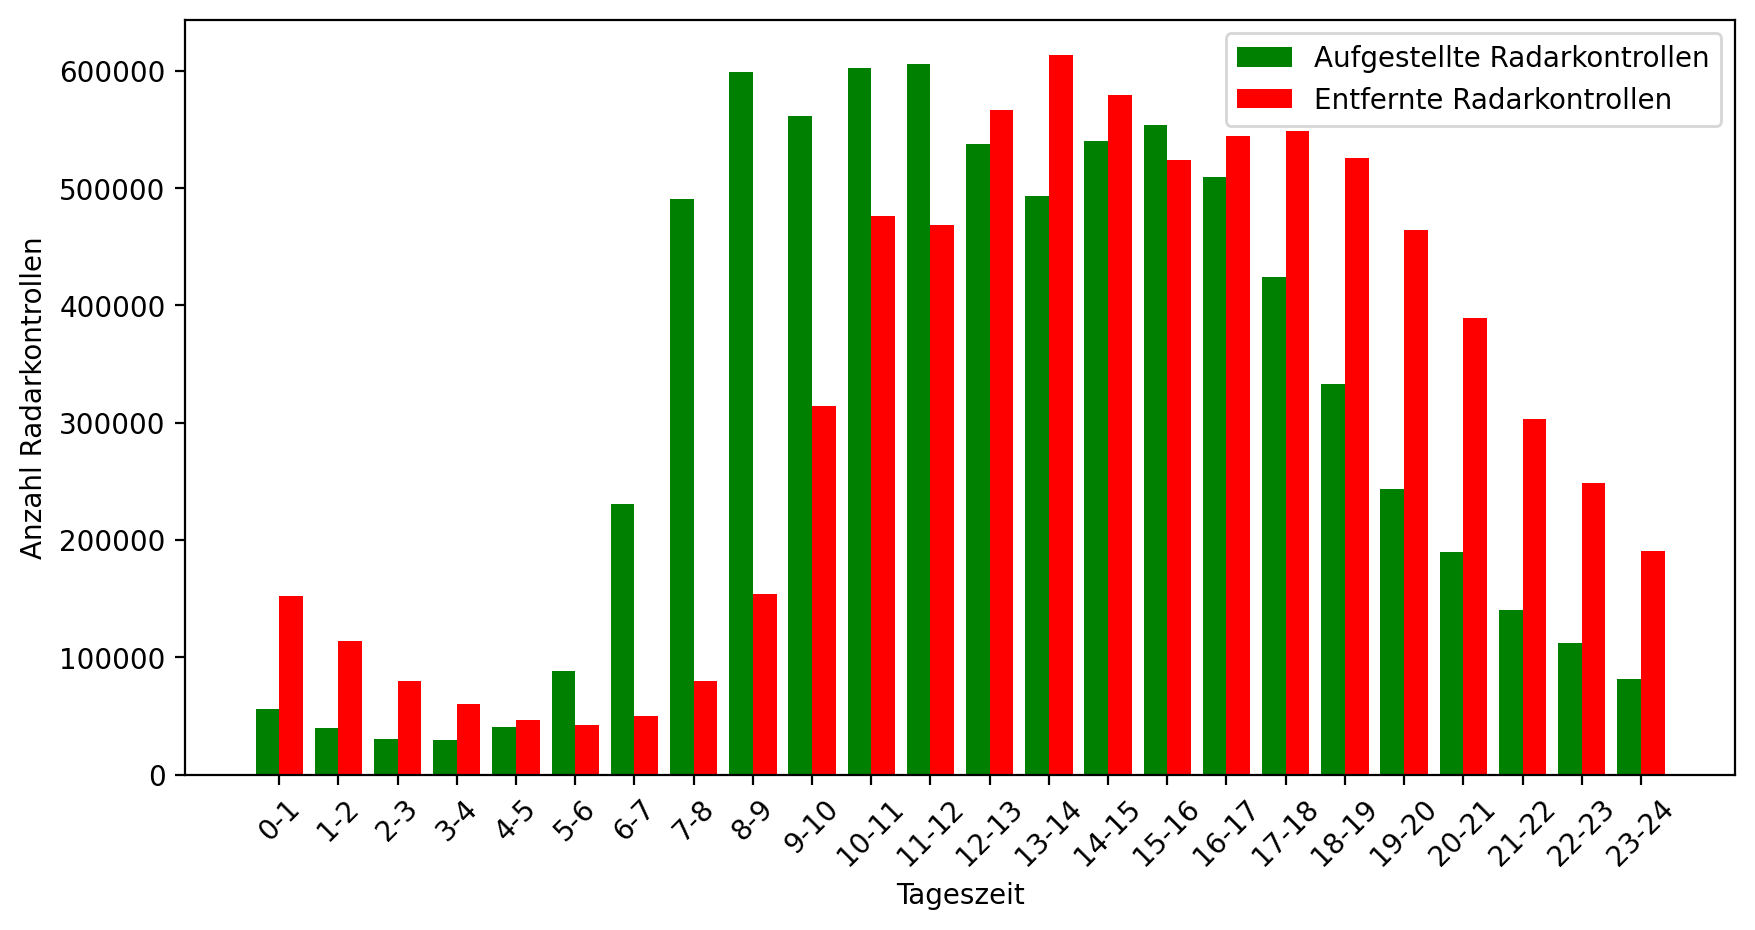
\includegraphics[width=1.0\textwidth,height=10cm,keepaspectratio=true]{content/images/AufbauAbbau.png}
    \caption{Auf- und Abbau mobiler Radarkontrollen nach Tageszeit}
    \label{fig:AufbauAbbauNachTageszeit}
\end{figure}

Wie erwartet kann man erkennen, dass zwischen 6 und 9 Uhr die Anzahl an neu gemeldeten Radarkontrollen stark ansteigt.
Es ist jedoch bemerkenswert, dass bis ca. 17 Uhr weiterhin viele Radarkontrollen neu gemeldet werden.
Gleichzeitig steigt bereits ab 9 Uhr die Anzahl an entfernten Meldungen stark an.
Von 12 bis 17 Uhr ist dann sowohl die Zahl an neuen und entfernten Meldungen konstant hoch.
Das bedeutet, dass die Radarkontrollen keineswegs den ganzen Tag an der gleichen Stelle stehen, sondern u.U. mehrmals am Tag umgestellt werden.
Daher ist die Gefahr, auf noch nicht gemeldete Radarkontrollen zu stoßen nicht nur morgens hoch, sondern auch tagsüber nicht zu vernachlässigen.
